\documentclass[11pt,a4paper]{article}

\usepackage[utf8]{inputenc}
\usepackage[T1]{fontenc}
\usepackage{lmodern}
\usepackage[english]{babel}
\usepackage[margin=2.6cm]{geometry}
\usepackage{microtype}
\usepackage{amsmath}
\usepackage{booktabs}
\usepackage{tabularx}
\usepackage{enumitem}
\usepackage{xcolor}
\usepackage{tikz}
\usetikzlibrary{arrows.meta,positioning}
\usepackage{pgfplots}
\pgfplotsset{compat=1.17}
\usepackage[hidelinks]{hyperref}

\setlist{itemsep=2pt,topsep=4pt}
\newcolumntype{R}{>{\raggedleft\arraybackslash}X}

\title{The Source Code of Law:\\
AI Agents Rewrite and Red-Team\\ Five Major Codes of French Law}

\author{
  Alex Masmejean\thanks{Corresponding author: \texttt{alex@masmej.com}.}\\
  \small Independent
  \and
  Kevin Primicerio\\
  \small Independent
}

\date{31 October 2026}

\begin{document}
\maketitle

\begin{abstract}
French law is hard to read: a single rule is spread across a statute, its implementing decrees, the tax annexes and future consolidated versions, which often contradict one another. We report a proof of concept in which AI agents rewrite, and then adversarially audit, five major French codes in full (the Labour Code, the General Tax Code and its four annexes, the Social Security Code, the Town Planning Code, and the Construction and Housing Code): 30{,}317 article entries from the official LEGI database as of 18 October 2026. Two drafting passes by orchestrated coding agents produced 14{,}115 rewritten articles and 16{,}199 articles retained with a specific justification. A third pass, run as an independent red team, built a register of objections (303 raised, 243 retained on the final text), applied about 1{,}220 corrections through a guarded writer with before-image checks, triaged issues filed by an external contributor, and measured reliability with six blind, stratified random audits. Over 1{,}879 randomly drawn articles, about 3.4\%\,$\pm$\,0.8 still carry a defect that a lawyer would notice, mostly dead or shifted cross-references, future versions that silently undo the reform, and decrees that keep obligations the statute removed. Targeted sweeps fix the family they aim at but do not move the measured rate; a systematic chapter-by-chapter reading of the 2{,}740 rewritten tax articles found 96 gross defects (3.5\%), 86 of which were corrected. The substantive choices follow the 2027 programme of David Lisnard, but the project is an independent initiative and the method is policy-agnostic. All texts, tools, audit samples and verdicts are public. No lawyer has validated the output.
\end{abstract}

\section{Introduction}

\paragraph{Legibility as a legal requirement.}
Accessibility and intelligibility of the law are an objective of constitutional value in France \cite{cc99421}. The Conseil d'État has for decades criticised the growth and instability of legal texts \cite{ce2016}.

The problem is not only the volume. A single rule is spread across several texts:
\begin{itemize}
  \item a statute (\emph{partie législative});
  \item its implementing decrees (\emph{partie réglementaire});
  \item for taxation, the four annexes of the CGI;
  \item consolidated future versions already published but not yet in force.
\end{itemize}
When one of these texts changes and the others do not, contradictions appear. Some are inherited from the official sources; others come from reform.

\paragraph{Origin of this work.}
On 19 October 2026 the first author published a short thread in French \cite{tweet}. It answered a public challenge and announced that AI agents had produced, overnight, rewritten versions of several French codes, published on five thematic websites. The thread invited lawyers, economists, employees and entrepreneurs to criticise the proposals article by article.

The reception was much larger than expected: about 120{,}000 views, 1{,}190 likes, 201 reposts and 293 bookmarks when last checked. The criticism that followed was more useful still. It made clear that a fast first draft was not enough, and that a credible demonstration needed three things:
\begin{enumerate}[label=(\roman*)]
  \item the complete codes, not a selection;
  \item a systematic search for contradictions;
  \item an honest measurement of what remains wrong.
\end{enumerate}
This paper documents that second, slower phase.

\paragraph{Goal.}
We pursue two goals.
\begin{itemize}
  \item \textbf{Legibility.} Produce, for every article in scope, a complete proposed text set side by side with the official source, with a written justification.
  \item \textbf{A proof of concept for contradiction finding and resolution.} Show how AI agents can find and resolve contradictions in a large, interconnected legal corpus, and how far that goes.
\end{itemize}
The second goal is the main scientific interest. Reforming a code is easy to state and hard to do consistently. Removing an obligation from a statute is meaningless if a decree, a tax annex or a future consolidated version keeps imposing it.

\paragraph{Contributions.}
\begin{itemize}
  \item A complete, versioned and public rewrite of nine legal instruments (30{,}317 entries). Official sources and proposals are kept apart, and a comparative reader and downloads are provided (\S\ref{sec:corpus}--\S\ref{sec:drafting}).
  \item A red-teaming protocol for AI-produced legislation:
  \begin{itemize}
    \item frozen, hashed snapshots;
    \item an objection register with priorities and natures;
    \item re-examination on diffs;
    \item correction under an explicit alignment criterion;
    \item a guarded writer that cannot silently overwrite (\S\ref{sec:redteam}).
  \end{itemize}
  \item A measurement method: six blind, stratified random audits, with a taxonomy of ten defect families (F1--F10). The rate has a confidence interval, not an anecdote (\S\ref{sec:measure}).
  \item Empirical findings on what AI agents do well and badly on legal coherence (\S\ref{sec:results}--\S\ref{sec:discussion}):
  \begin{itemize}
    \item mechanical sweeps reach a plateau;
    \item correction rounds can create new defects;
    \item a large part of the residual error comes from texts outside the corpus.
  \end{itemize}
\end{itemize}

\paragraph{Political stance.}
The substantive orientation of the rewrite is explicit and is not neutral. It aims at fewer taxes and constraints. It keeps exemptions, favourable derogations, acquired rights and transitions. It never introduces a replacement formality.

These choices are inspired by the 2027 programme of David Lisnard \cite{lisnard}. \textbf{This project is an independent initiative.} It is not commissioned, reviewed or endorsed by David Lisnard or by his movement, Nouvelle Énergie, and the published websites say so.

The method is policy-agnostic. The policy layer is a separate, explicit input (\S\ref{sec:policy}), and the same pipeline could implement any other programme. The red team was instructed to fix contradictions and loopholes, \emph{never} to change political choices.

\section{Related work}

Large language models are increasingly evaluated on legal reasoning, e.g.\ LegalBench \cite{legalbench}. Work on making legislation machine-readable comes in two forms:
\begin{itemize}
  \item programming languages for statutes, such as Catala, applied to French tax law \cite{catala};
  \item ``rules as code'' initiatives \cite{oecd2020}.
\end{itemize}
Both formalise existing law faithfully. Our goal is different: we \emph{rewrite} the law according to a reform programme, and then check the coherence of the result.

Red-teaming, the adversarial search for failures by an independent party, is standard practice for AI systems \cite{ganguli2022}. Here it is turned against AI-produced legislation.

We are not aware of prior work that rewrites complete national codes end to end and publishes a measured defect rate.

\section{Corpus and scope}
\label{sec:corpus}

The corpus is frozen at \textbf{18 October 2026}. It is built from the official LEGI database of the Direction de l'information légale et administrative (DILA) \cite{legi}: the stock of 13 July 2025, plus 466 daily updates.

The working identity of an article is the pair (code identifier, version identifier \texttt{LEGIARTI}), together with a hash of its source and its validity dates. Numbers alone are never trusted, because they are recycled. The database holds 135{,}904 historical versions; the scope is the 30{,}317 entries in force or scheduled (Table~\ref{tab:corpus}).

\begin{table}[ht]
\centering
\small
\begin{tabularx}{\linewidth}{lRRRR}
\toprule
Instrument & Entries & Rewritten & Retained & Reserves\\
\midrule
Labour Code & 11{,}593 & 4{,}296 & 7{,}297 & 0\\
General Tax Code (CGI) & 2{,}375 & 1{,}387 & 988 & 0\\
Social Security Code & 7{,}427 & 3{,}178 & 4{,}247 & 2\\
Town Planning Code & 2{,}459 & 1{,}530 & 929 & 0\\
Construction and Housing Code & 4{,}126 & 2{,}205 & 1{,}921 & 0\\
CGI annex I & 71 & 42 & 29 & 0\\
CGI annex II & 674 & 388 & 286 & 0\\
CGI annex III & 1{,}115 & 799 & 316 & 0\\
CGI annex IV & 477 & 290 & 186 & 1\\
\midrule
Total & 30{,}317 & 14{,}115 & 16{,}199 & 3\\
\bottomrule
\end{tabularx}
\caption{Scope at the end of the second pass. ``Retained'' articles are kept unchanged with a specific justification. The three ``reserves'' are documentary gaps (a missing figure, missing original forms, and a conflict in the official consolidation) that were not filled by guesswork.}
\label{tab:corpus}
\end{table}

Out of scope are texts that the corpus cites but does not contain. Examples are the Monetary and Financial Code, the Commercial Code, non-codified statutes, ministerial orders, and the Code of taxes on goods and services (CIBS), into which much of VAT is being recodified on 1 January 2027. This boundary turns out to matter (\S\ref{sec:discussion}).

\section{Drafting pipeline (first and second passes)}
\label{sec:drafting}

\begin{figure}[ht]
\centering
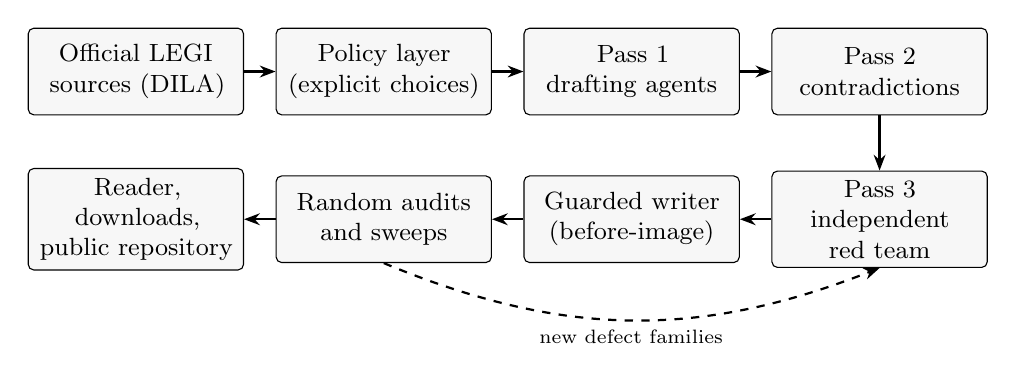
\begin{tikzpicture}[node distance=3mm and 4mm, font=\small,
  box/.style={draw, rounded corners=2pt, align=center, minimum height=11mm, text width=25mm, fill=gray!6},
  arr/.style={-{Stealth[length=2mm]}, thick}]
\node[box] (src) {Official LEGI\\sources (DILA)};
\node[box, right=of src] (pol) {Policy layer\\(explicit choices)};
\node[box, right=of pol] (p1) {Pass 1\\drafting agents};
\node[box, right=of p1] (p2) {Pass 2\\contradictions};
\node[box, below=7mm of p2] (rt) {Pass 3\\independent red team};
\node[box, left=of rt] (fix) {Guarded writer\\(before-image)};
\node[box, left=of fix] (aud) {Random audits\\and sweeps};
\node[box, left=of aud] (pub) {Reader, downloads,\\public repository};
\draw[arr] (src) -- (pol); \draw[arr] (pol) -- (p1); \draw[arr] (p1) -- (p2);
\draw[arr] (p2) -- (rt); \draw[arr] (rt) -- (fix); \draw[arr] (fix) -- (aud);
\draw[arr] (aud) -- (pub);
\draw[arr, dashed] (aud.south) to[bend right=22] node[below, font=\scriptsize]{new defect families} (rt.south);
\end{tikzpicture}
\caption{Overview of the pipeline. Every write goes through the same guarded writer; audits feed new defect families back to the red team.}
\label{fig:pipeline}
\end{figure}


\subsection{Policy layer}
\label{sec:policy}

Figure~\ref{fig:pipeline} summarises the whole pipeline. All substantive decisions are stored as explicit, versioned policy objects, separate from the legal text: per-domain coordinations, site summaries, and a net-costing method for tax measures. Examples:
\begin{itemize}
  \item a single open-ended employment contract with a 15-day notice period on each side;
  \item corporate tax triggered by distribution;
  \item abolition of inheritance taxes, while gifts remain taxed;
  \item abolition of production taxes;
  \item shorter planning-permit deadlines.
\end{itemize}
The rest of the pipeline treats them as inputs.

Editorial invariants apply throughout:
\begin{itemize}
  \item official sources are never overwritten;
  \item no rate, date, equivalence or facsimile is invented;
  \item favours are never removed to make two texts artificially consistent;
  \item an obligation removed in a statute must not survive in a decree, a form or a cross-reference.
\end{itemize}

\subsection{Article-level workers}

Each article (or batch of related articles) is processed by a non-interactive coding agent. The agent receives:
\begin{itemize}
  \item the complete source XML, including notes (\emph{NOTA}), tables and versions;
  \item the applicable policies;
  \item the explicit cross-reference targets.
\end{itemize}
It must return the \emph{complete} proposed article, never a summary, together with a reason and review notes. It assigns one of two statuses, \texttt{rewrite\_draft} or \texttt{retained\_unchanged}. Repeals and partial reductions are typed (\texttt{full\_repeal}, \texttt{normative\_reduction}). Every removed provision is listed, so that a reduction is auditable.

The first pass used an OpenAI model (\texttt{gpt-6-astra}, medium effort) through the Codex command-line agent. The second pass used \texttt{gpt-6.1-sol} at high effort.

\subsection{Second pass: contradictions first}

From 23 October, the priority shifted from further cuts to \emph{contradictions and inconsistencies}, within an article, between articles and across the nine instruments. All 30{,}314 prior drafts were re-read against their complete sources and counterparts. Each worker classified every tension it found as one of:
\begin{itemize}
  \item an effective contradiction;
  \item a required coordination;
  \item a compatible transition;
  \item a difference of scope;
  \item a point that cannot be verified.
\end{itemize}

\subsection{Guards}

Nothing is accepted on the word of a model. An answer is accepted only after the following checks:
\begin{itemize}
  \item source, NOTA and validity dates;
  \item content validation, including allowed markup and complete tables;
  \item a before-image check on five canonical fields (source hash, status, proposal, reason, notes), both in the database and in the batch file that owns the article;
  \item ownership, registry and archive;
  \item an independent whole-corpus validation.
\end{itemize}
Native execution evidence (model, effort, session) is also checked.

These guards are not decoration. They caught real divergences: three second-pass jobs were refused because the article had changed under them. The guards also made the third pass possible, because every correction could be applied through the same writer.

The second pass ended on 29 October with all 30{,}314 identities accepted. A post-hoc structural audit then listed 94{,}059 points to examine, 1{,}412 of them high-priority, on 792 articles. These are leads, not established contradictions.

\section{Independent red team (third pass)}
\label{sec:redteam}

The third pass was run with a different system, Anthropic's Claude Code (Claude Opus 5.5). A coordinating agent dispatched about 390 sub-agent runs over five days. It worked as an \emph{independent} reviewer, under strict rules:
\begin{itemize}
  \item read-only access to production, on frozen snapshots whose files are all hashed;
  \item exact quotations with version identifiers for every claim;
  \item no invented source, date or ``evidence of resolution'';
  \item no bypass of access controls;
  \item an explicit statement that an AI review is not a lawyer's validation.
\end{itemize}

\subsection{Objection register}

The first wave covered 31 thematic dossiers (for example future versions, decrees versus statutes, tax annexes, and the transitions of the 2026 occupational-injury reform). Five priority domains followed: distribution-based corporate tax, inheritance, the SRU social-housing quotas, the CVAE production tax, and the payroll tax.

Each objection records:
\begin{itemize}
  \item a priority: P0 (grave and certain effect), P1 (probable effect) or P2 (limited effect);
  \item a nature: missing coordination, inconsistency introduced by the project, legal risk, source conflict, inventory anomaly, documentary reserve or simple alert;
  \item the exact passages, the reasoning and a \emph{minimal correction};
  \item what must be preserved: rights, favours and transitions.
\end{itemize}
The 1{,}943 structural alerts given high priority by the static audit were classified one by one. Duplicates were merged with a written reason (46 merges).

\subsection{Re-examination on diffs}

The second pass was still running when the red team started. The register was therefore re-examined twice, against an intermediate snapshot and then the final one, using a file-level diff. On the final text, 136 objections whose articles had changed were re-read:
\begin{itemize}
  \item 58 were resolved by the second pass (including 17 P1);
  \item 30 were reformulated;
  \item 48 were maintained.
\end{itemize}
The final register holds \textbf{243 objections}: 3 P0, 83 P1 and 157 P2, of which 188 are confirmed and 55 still to be confirmed.

\subsection{From review to correction}

After the review, the first author made the red team the sole writer, with one standing instruction: issues may fix contradictions and loopholes, never political choices. A correction is applied only if it does one of three things:
\begin{enumerate}[label=(\alph*)]
  \item make a decided reform effective, for example by carrying it onto a published future version that would otherwise restore the old rule;
  \item remove a contradiction;
  \item close a loophole that contradicts the declared object of the project.
\end{enumerate}
A correction is refused if it does any of the following:
\begin{itemize}
  \item create or raise a tax;
  \item add a formality or a condition;
  \item remove an exemption or an acquired right;
  \item reverse an explicit choice of the author;
  \item settle an open political question.
\end{itemize}

Drafting agents write corrections only in a workspace, as complete article texts with typed metadata. A checker rebuilds each row exactly as the production applier would and runs the project's own validator in a temporary directory.

The coordinator then applies the corrections with the guarded tool. That tool checks the before-image, archives the old text, revalidates the whole corpus and rolls back on failure. An ownership map gives each article to a single group. Cross-group needs are expressed as requests, so two agents never write the same article.

\subsection{External contributions}

During the review, an external contributor (the second author) filed 13 issues and two pull requests on the public repository. These were produced with his own AI agents and covered labour-law cross-references, decrees that survive repealed statutes, penalties and works-council committees. Each issue was triaged against the register on the current text. Three of the issues asked for policy changes; they were explained and closed as not planned.

\section{Measuring reliability}
\label{sec:measure}

A register says what was found, not what remains. We therefore measured the residual defect rate directly.

\paragraph{Sampling.}
Each audit draws about 314 articles at random. The draw is stratified by instrument and by level (statute or regulation), and each stratum gets at least six articles. Successive audits exclude every article read before. Seeds are published.

\paragraph{Blind reading.}
Ten agents per audit read their share ``as a lawyer would'', on the production text: the article, its future versions, its three most important links, and its implementing texts or legal basis. They do not consult the register before qualifying an article.

\paragraph{Verdicts.}
Each article is classified as:
\begin{itemize}
  \item \textbf{G} (gross): a lawyer would notice it and find it abnormal;
  \item \textbf{m} (minor): wrong notes, clumsy but harmless wording, or a reasonable doubt;
  \item \textbf{0}: nothing to report.
\end{itemize}
Each G or m needs an exact quotation. Rates are weighted by stratum, with 95\% intervals. Defects are classified into ten families:

\begin{table}[ht]
\centering
\small
\begin{tabularx}{\linewidth}{lX}
\toprule
F1 & A statute removes a formality or an obligation, but a decree or an annex still organises it.\\
F2 & A penalty survives the obligation it punishes.\\
F3 & Dead, shifted or wrong cross-reference.\\
F4 & A published future version, with no proposal, restores the old rule; or a false claim that an article is repealed.\\
F5 & Contradiction between two provisions (other than F1).\\
F6 & Missing or faulty transition (retroactivity, loss of acquired rights).\\
F7 & Defective text (truncated, broken numbering, amputated table).\\
F8 & Contrary to a declared orientation (a tax or formality re-created, a favour removed without decision).\\
F9 & Higher-law risk (Constitution, EU law), always ``to be confirmed''.\\
F10 & Notes or reasons only (always minor).\\
\bottomrule
\end{tabularx}
\caption{Defect families used by auditors and sweeps.}
\label{tab:families}
\end{table}

\paragraph{Family sweeps.}
After each audit, we turned its gross defects into mechanical lead generators and swept the whole corpus for them. Examples:
\begin{itemize}
  \item a decree citing a repealed statute;
  \item a penalty citing a removed article;
  \item a reference to the $n$-th paragraph of an article that a proposal or future version has shifted;
  \item a current version with a proposal whose next published version has none;
  \item a decree that still uses the distinctive words of what its statute removed;
  \item a chapter where only some articles are repealed.
\end{itemize}
Leads are not findings. Each lead is qualified by an agent that reads the texts in full, as a false positive, already fixed, G or m. A correction is drafted for every confirmed G.

\paragraph{Systematic reading.}
Finally, we read every rewritten article of the CGI and its annexes, where the audits showed the highest rates. The 2{,}740 articles not already audited were grouped by their deepest section, so that each reader sees a whole chapter. They were split into 132 packets of about 21 articles. Each reader qualifies every article and drafts corrections for its gross defects.

\section{Results}
\label{sec:results}

\subsection{Corrections applied}

Over five days, the third pass applied \textbf{1{,}222 correction rows to 1{,}151 distinct articles}:
\begin{itemize}
  \item 966 replacements of existing proposals;
  \item 256 new proposals on published future versions, which would otherwise have restored the pre-reform text when they enter into force.
\end{itemize}
Each row was validated by the project's own validator and archived with before and after hashes. The project's 321 tests pass after every round. Table~\ref{tab:rounds} breaks the rows down by source.

\begin{table}[ht]
\centering
\small
\begin{tabularx}{\linewidth}{Xrr}
\toprule
Source of corrections & Leads or objections & Rows applied\\
\midrule
P0/P1 objections and first GitHub issues & 86 objections & 395\\
P2 objections & 157 objections & 201\\
Sweep 1 (dead references, future versions) & 1{,}127 leads $\rightarrow$ 154 G & 145\\
Sweep 2 (statute removes, decree keeps) & 1{,}117 leads $\rightarrow$ 33 G & 36\\
Audit 1--3 defects, notes pilot, later issues & -- & $\approx$ 90\\
Round 4 (audit 4 + sweep) & 918 leads $\rightarrow$ 45 G & 64\\
Round 5 (audit 5 + tax-aware sweep) & 548 leads $\rightarrow$ 114 G & 97\\
Round 6 (audit 6 + whole chapters) & 365 leads $\rightarrow$ 25 G & 110\\
Systematic reading, CGI and annexes & 2{,}740 articles $\rightarrow$ 96 G & 81\\
\bottomrule
\end{tabularx}
\caption{Corrections applied by the third pass, by source. Counts come from the per-round reports; the ``$\approx$'' line groups small fix sets.}
\label{tab:rounds}
\end{table}

\subsection{Residual defect rate}

\begin{table}[ht]
\centering
\small
\begin{tabular}{lrrrr}
\toprule
Audit (state of the text) & Sample & G & G rate & G or m\\
\midrule
1 (after P0/P1 corrections) & 309 & 12 & 4.0\% $\pm$ 2.2 & 21.1\%\\
2 (after sweep 1) & 314 & 9 & 2.9\% $\pm$ 1.9 & 22.1\%\\
3 (after sweep 2) & 314 & 12 & 3.8\% $\pm$ 2.1 & 17.7\%\\
4 (after P2 objections) & 314 & 8 & 2.5\% $\pm$ 1.7 & 14.6\%\\
5 (after round 4) & 314 & 10 & 3.2\% $\pm$ 1.9 & 22.6\%\\
6 (after round 5) & 314 & 13 & 4.1\% $\pm$ 2.2 & 15.3\%\\
\midrule
Pooled & 1{,}879 & 64 & \textbf{3.4\% $\pm$ 0.8} & \\
\bottomrule
\end{tabular}
\caption{Six independent blind random audits. Each sample excludes all previously read articles.}
\label{tab:audits}
\end{table}

\begin{figure}[ht]
\centering
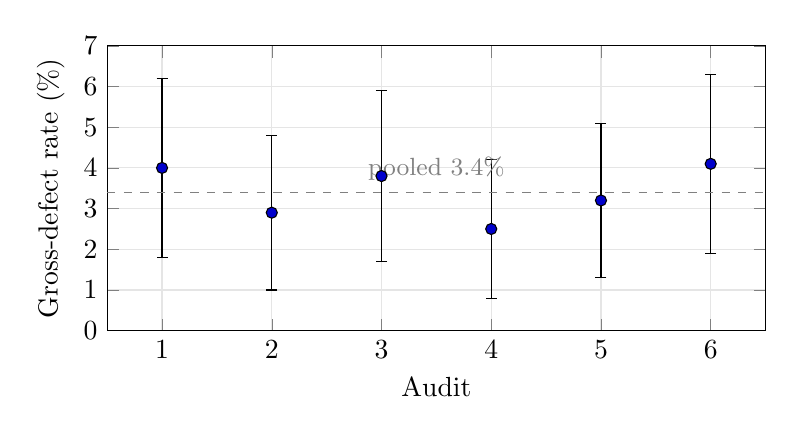
\begin{tikzpicture}
\begin{axis}[
  width=0.82\linewidth, height=5.2cm,
  xlabel={Audit}, ylabel={Gross-defect rate (\%)},
  xmin=0.5, xmax=6.5, ymin=0, ymax=7,
  xtick={1,2,3,4,5,6}, ytick={0,1,2,3,4,5,6,7},
  grid=major, grid style={gray!20},
]
\addplot+[only marks, mark=*, black, error bars/.cd, y dir=both, y explicit]
  coordinates {(1,4.0) +- (0,2.2) (2,2.9) +- (0,1.9) (3,3.8) +- (0,2.1)
               (4,2.5) +- (0,1.7) (5,3.2) +- (0,1.9) (6,4.1) +- (0,2.2)};
\addplot[dashed, gray, domain=0.5:6.5] {3.4};
\node[anchor=south, font=\small, gray] at (axis cs:3.5,3.45) {pooled 3.4\%};
\end{axis}
\end{tikzpicture}
\caption{Measured gross-defect rate per audit, with 95\% intervals. No decline can be detected from one round to the next.}
\label{fig:audits}
\end{figure}

About 3.4\% of articles (95\% interval 2.6--4.2\%) still carry a gross defect (Table~\ref{tab:audits}, Figure~\ref{fig:audits}). Put differently, a lawyer who reads 20 articles in their field has roughly an even chance of meeting at least one.

The rate shows no measurable decline from round to round, even though each round fixed 50 to 110 articles. This is expected. If about 1{,}000 articles are defective, fixing 100 lowers the rate by about 0.3 points, well below what a 314-article audit can detect ($\pm$2 points).

The composition of the defects did change:
\begin{itemize}
  \item after the first sweep, dead references (F3) receded;
  \item contradictions between two proposals (F5) moved to the top;
  \item later audits concentrated on the tax annexes.
\end{itemize}
Of the gross defects found by audits, between half and three quarters were unknown to the register.

\subsection{Sweeps: yield and plateau}

Sweep yields fell as each family was exhausted. The ``statute removes, decree keeps'' sweep reached 3\% G per lead, against 14\% for the first sweep. Only re-qualification brought the yield back up: when earlier minor leads were re-read at the audit threshold, 56 of 166 turned out to be gross.

A pilot on 250 articles whose review notes announced an open coordination found that 60\% of such notes were simply outdated. Its G rate was 4.8\%, barely above random reading, so the full sweep was not run.

\subsection{Systematic reading of the tax code}

The chapter-by-chapter reading of the 2{,}740 rewritten CGI and annex articles gave:
\begin{itemize}
  \item 96 gross defects (3.5\%);
  \item 383 minor defects;
  \item 2{,}261 articles with nothing to report.
\end{itemize}
The 3.5\% is far below the 9--12\% that the pooled audits suggested for these strata. Those estimates rested on small samples (76 and 128 articles), and rounds 4 to 6 had concentrated on the tax annexes. We cannot exclude that a reader going through a whole chapter is somewhat less strict than a blind auditor.

Of the 96 defects, 86 are corrected (81 rows, 16 of them requested across groups). Ten remain open. Nine are VAT reforms written into CGI subdivisions that a 2025 ordinance moves to the CIBS on 1 January 2027, so the reforms would have no effect; the CIBS is outside the corpus. The tenth is a political arbitration left to the author.

The reading consumed about 30 million tokens (excluding cache reads), roughly 11{,}000 tokens per article.

\subsection{Examples of defects}

The following examples, all corrected unless stated otherwise, show the kind of errors AI drafting produces and AI review can catch:
\begin{itemize}
  \item \emph{Re-creating a tax the project abolishes.} The inventory had selected a version of CGI 1609 \emph{quinvicies} that never entered into force. Its proposal re-instituted the additional apprenticeship contribution that the proposed Labour Code L6242-1 abolishes.
  \item \emph{A ``reduced'' rate above the normal rate.} After the corporate-tax reform, the reduced 24\% rate for non-profit bodies (CGI 219 \emph{bis}) exceeded the new normal rate of 20\%.
  \item \emph{Half-repealed chapters.} In CGI annex II, a correction round repealed some articles on approved management centres, whose legal basis (CGI 1649 \emph{quater} C to O) had been repealed in 2025. Neighbouring articles still organised the approval procedure. The next audit caught it, and the whole chapter was then treated at once.
  \item \emph{Future versions undoing the reform.} A Mayotte adaptation scheduled for 2028 (Social Security Code L759-23) applied ``in the following wording'' an article that the project rewrote, and so restored the rule the project removes.
  \item \emph{A regulation against its statute.} A proposed tax decree dropped the prior accreditation of fiscal representatives, while the statute (CGI 1671) still required it. The coherent fix aligns the statute instead of restoring a formality.
\end{itemize}

\section{Discussion}
\label{sec:discussion}

\paragraph{What AI agents do well.}
At this scale, agents are tireless, complete and literal readers. They reproduce full articles, including tables of several hundred thousand characters. They follow cross-references through nine instruments and many versions, and they keep exact quotations. Combined with typed changes and guarded writes, this made it possible to rewrite and then repair a corpus that no individual could re-read in a week. It also made the work fully auditable: every change is archived with its before-image and its reason.

\paragraph{What they do badly.}
\begin{itemize}
  \item \emph{The boundary of the corpus.} Many defects involve a text that was not provided: the CIBS, non-codified statutes, ministerial orders. An agent can only flag them as documentary reserves, and must not guess.
  \item \emph{Time.} Legal texts have scheduled future versions. A reform written on a version that ends before the reform can take effect is void. A future version with no proposal silently restores the old rule.
  \item \emph{Local coherence without global coherence.} A single change is valid in isolation, but its neighbours are left inconsistent. One of our own correction rounds created exactly such a half-repealed chapter. We fixed this by treating whole chapters at once and by running a regression check after each application: any article still citing an article repealed in the round.
  \item \emph{Calibration.} Readers differ in how strictly they separate gross from minor. Early sweeps under-rated dead references as minor. Re-qualifying them at the audit threshold turned a third of them into gross defects.
\end{itemize}

\paragraph{Measurement changes the conversation.}
Without the random audits, the number of corrections, over 1{,}200, would have suggested steady progress. The audits show a plateau around 3--4\%, and they explain it. Targeted sweeps help, but the remaining defects are scattered. Only systematic reading can bring the rate clearly down. We consider a published, reproducible defect rate with an interval the minimum standard for any claim about AI-drafted legislation.

\paragraph{Contradictions versus politics.}
Keeping the red team away from political choices was harder than expected. Many apparent contradictions have two coherent resolutions: removing a favour or extending it, restoring a formality or deleting its remnant. We resolved this with an explicit, published alignment criterion (\S\ref{sec:redteam}), and we sent genuine arbitrations back to the author. A different programme would change the criterion, not the method.

\paragraph{Human review.}
No lawyer has validated the output. The pipeline makes legal review \emph{cheaper}, not unnecessary: each article comes with its source, reason, notes, objections and audit trail. The public issue tracker turned out to be the most efficient channel. Nine of the first eleven external issues pointed at a real defect.

\section{Limitations}

\begin{itemize}
  \item AI review is not legal validation. Audit verdicts are model judgements and may be wrong in either direction.
  \item The corpus is frozen at 18 October 2026, and texts outside the nine instruments are not rewritten.
  \item Audit samples of about 314 articles detect changes of about $\pm$2 points only, so per-stratum rates are imprecise.
  \item The drafting models and the reviewing model come from different vendors, which limits shared blind spots but does not remove them.
  \item Costs were not tracked uniformly across passes, and productivity claims would be speculative.
  \item The economic and fiscal effects of the reform are outside the scope of this paper.
\end{itemize}

\section{Conclusion and future work}

We rewrote five French codes and the four CGI annexes end to end with AI agents, red-teamed the result independently, and measured what remains wrong. The residual gross-defect rate is about 3.4\%, and the full trail is public.

Next steps:
\begin{itemize}
  \item systematic reading of the remaining rewritten articles: the housing and social security codes (about 5{,}500), then labour and town planning (about 5{,}900);
  \item bringing the CIBS into the corpus;
  \item validation by practising lawyers, starting with the open objections and arbitrations.
\end{itemize}
Beyond this particular reform, the method is a template: an explicit policy layer, complete drafting, guarded writes, an independent red team and honest measurement. We hope it makes the law more legible, and that it gives anyone a concrete way to check whether a proposed reform is coherent.

\section*{Data and code availability}

The rewritten corpus, the official sources, policies, batches, the third-pass reports and register, the audit samples and verdicts, and the sweep and reading tools are public at \url{https://github.com/AlexMasmej/liberer-la-france}. A comparative reader and complete downloads are at \url{https://www.libererlaretraite.com/corpus/} and \url{https://www.libererlaretraite.com/telechargements/}.

\section*{Use of AI}

AI systems did most of the drafting, reviewing and correction work described here, under human direction and arbitration. This manuscript was drafted with the assistance of Claude (Anthropic) from the project's records and reviewed by the authors.

\section*{Author contributions}

A.M.\ conceived and directed the project, set the policy layer, ran the drafting passes and arbitrated all political choices. K.P.\ conducted an independent external review of the published codes with his own AI agents, filing issues and acceptance tests that were triaged and partly integrated. Both authors reviewed the manuscript.

\section*{Acknowledgements}

We thank Rand Hindi for the inspiration behind the red-teaming approach of the third pass. We thank everyone who read, criticised and shared the initial thread.

\begin{thebibliography}{99}

\bibitem{cc99421}
Conseil constitutionnel,
Décision n\textsuperscript{o} 99-421 DC du 16 décembre 1999, \emph{Loi portant habilitation du Gouvernement à procéder, par ordonnances, à l'adoption de la partie législative de certains codes}.

\bibitem{ce2016}
Conseil d'État,
\emph{Simplification et qualité du droit}, Étude annuelle 2016, La Documentation française, 2016.

\bibitem{tweet}
A.~Masmej,
Thread on X, 19 October 2026,
\url{https://x.com/AlexMasmej/status/2112088220804722917} (engagement figures read on 31 October 2026).

\bibitem{lisnard}
D.~Lisnard and Nouvelle Énergie,
Programme for the 2027 French presidential election,
\url{https://www.unenouvelleenergie.fr/}.

\bibitem{legi}
Direction de l'information légale et administrative (DILA),
LEGI: codes, lois et règlements consolidés,
\url{https://www.data.gouv.fr/datasets/legi-codes-lois-et-reglements-consolides}.

\bibitem{legalbench}
N.~Guha et al.,
LegalBench: A collaboratively built benchmark for measuring legal reasoning in large language models,
\emph{NeurIPS Datasets and Benchmarks}, 2023. arXiv:2308.11462.

\bibitem{catala}
D.~Merigoux, N.~Chataing and J.~Protzenko,
Catala: A programming language for the law,
\emph{Proceedings of the ACM on Programming Languages} 5(ICFP), 2021. arXiv:2103.03198.

\bibitem{oecd2020}
OECD Observatory of Public Sector Innovation,
\emph{Cracking the Code: Rulemaking for Humans and Machines}, OECD, 2020.

\bibitem{ganguli2022}
D.~Ganguli et al.,
Red teaming language models to reduce harms: Methods, scaling behaviors, and lessons learned,
arXiv:2209.07858, 2022.

\end{thebibliography}

\end{document}
